\documentclass{beamer}

\usepackage[ruled]{algorithm2e}
\SetKw{KwRet}{return}
\usepackage{amsmath}

\usetheme{AnnArbor}
\usecolortheme{crane}
\usefonttheme[onlymath]{serif}

\title{Deep Learning - Foundations and Concepts}
\subtitle{Chapter 8. Backpropagation}
\author{nonlineark@github}
\date{\today}

\begin{document}

\begin{frame}
    \titlepage
\end{frame}

\begin{frame}
    \frametitle{Outline}
    \tableofcontents
\end{frame}

\section{Evaluation of Gradients}

\begin{frame}
    \frametitle{Single-layer networks}
    Consider a simple linear model:
    \begin{equation*}
        y_{k}=\sum_{i}w_{ki}x_{i}
    \end{equation*}
    together with a sum-of-squares error function:
    \begin{equation*}
        E_{n}=\frac{1}{2}\sum_{k}(y^{n}_{k}-t^{n}_{k})^{2}
    \end{equation*}
    The gradient of this error function with respect to a weight $w_{ji}$ is given by:
    \begin{equation*}
        \frac{\partial{}E_{n}}{\partial{}w_{ji}}=\frac{1}{2}\sum_{k}2(y^{n}_{k}-t^{n}_{k})\frac{\partial{}y^{n}_{k}}{\partial{}w_{ji}}=(y^{n}_{j}-t^{n}_{j})x^{n}_{i}
    \end{equation*}
    This is a local computation involving:
    \begin{itemize}
        \item An error signal $y^{n}_{j}-t^{n}_{j}$ associated with the output end.
        \item The variable $x^{n}_{i}$ associated with the input end.
    \end{itemize}
\end{frame}

\begin{frame}
    \frametitle{General feed-forward networks}
    Consider a unit in a feed-forward network:
    \begin{equation*}
        a_{j}=\sum_{i}w_{ji}z_{i}\qquad{}z_{j}=h(a_{j})
    \end{equation*}
    Now consider the evaluation of the derivative of $E_{n}$ with respect to a weight $w_{ji}$:
    \begin{equation*}
        \frac{\partial{}E_{n}}{\partial{}w_{ji}}=\sum_{k}\frac{\partial{}E_{n}}{\partial{}a_{k}}\frac{\partial{}a_{k}}{\partial{}w_{ji}}=\frac{\partial{}E_{n}}{\partial{}a_{j}}\frac{\partial{}a_{j}}{\partial{}w_{ji}}
    \end{equation*}
    If we introduce $\delta_{j}=\frac{\partial{}E_{n}}{\partial{}a_{j}}$, and use the fact that $\frac{\partial{}a_{j}}{\partial{}w_{ji}}=z_{i}$, we have:
    \begin{equation*}
        \frac{\partial{}E_{n}}{\partial{}w_{ji}}=\delta_{j}z_{i}
    \end{equation*}
    This takes the same form as that found for the simple linear model.
\end{frame}

\begin{frame}
    \frametitle{General feed-forward networks}
    To evaluate the derivatives, we need calculate only the value of $\delta_{j}$ for each hidden and output unit. For output units:
    \begin{equation*}
        \delta_{j}=\frac{\partial{}E_{n}}{\partial{}a_{j}}=\sum_{k}\frac{\partial{}E_{n}}{\partial{}y_{k}}\frac{\partial{}y_{k}}{\partial{}a_{j}}=y_{j}-t_{j}
    \end{equation*}
    provided we are using the canonical link as the output-unit activation function. For hidden units:
    \begin{equation*}
        \delta_{j}=\frac{\partial{}E_{n}}{\partial{}a_{j}}=\sum_{k}\frac{\partial{}E_{n}}{\partial{}a_{k}}\frac{\partial{}a_{k}}{\partial{}a_{j}}=\sum_{k}\frac{\partial{}E_{n}}{\partial{}a_{k}}\frac{\partial{}a_{k}}{\partial{}z_{j}}\frac{\mathrm{d}z_{j}}{\mathrm{d}a_{j}}=h'(a_{j})\sum_{k}w_{kj}\delta_{k}
    \end{equation*}
    which tells us that the value of $\delta$ for a particular hidden unit can be obtained by propagating the $\delta$'s backwards from units higher up in the network.
\end{frame}

\begin{frame}
    \frametitle{General feed-forward networks}
    \begin{figure}
        \caption{Illustration of the calculation of $\delta_{j}$ for hidden unit $j$}
        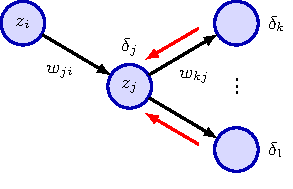
\includegraphics{Figure_1.pdf}
    \end{figure}
\end{frame}

\begin{frame}
    \frametitle{General feed-forward networks}
    \begin{algorithm}[H]
        \caption{Backpropagation}
        \For{$j\in$ all hidden and output units}{
            $a_{j}\gets\sum_{i}w_{ji}z_{i}$\;
            $z_{j}\gets{}h(a_{j})$\;
        }
        \For{$k\in$ all output units}{
            $\delta_{k}\gets\frac{\partial{}E_{n}}{\partial{}a_{k}}$\;
        }
        \For{$j\in$ all hidden units}{
            $\delta_{j}\gets{}h'(a_{j})\sum_{k}w_{kj}\delta_{k}$\;
            $\frac{\partial{}E_{n}}{\partial{}w_{ji}}\gets\delta_{j}z_{i}$\;
        }
        \Return{$\nabla{}E_{n}$}\;
    \end{algorithm}
\end{frame}

\begin{frame}
    \frametitle{Numerical differentiation}
    One of the most important aspects of backpropagation is its $\mathcal{O}(W)$ computational efficiency. Consider an alternative approach to use finite differences with:
    \begin{equation*}
        \frac{\partial{}E_{n}}{\partial{}w_{ji}}\approx\frac{E_{n}(w_{ji}+\epsilon)-E_{n}(w_{ji})}{\epsilon}
    \end{equation*}
    or use symmetrical central differences for better accuracy of the approximation:
    \begin{equation*}
        \frac{\partial{}E_{n}}{\partial{}w_{ji}}\approx\frac{E_{n}(w_{ji}+\epsilon)-E_{n}(w_{ji}-\epsilon)}{2\epsilon}
    \end{equation*}
    There are $W$ weights in the network each of which must be perturbated individually, so that the overall computational cost is $\mathcal{O}(W^{2})$.
\end{frame}

\begin{frame}
    \frametitle{The Jacobian matrix}
    Here we consider the network outputs as a function of the network inputs, and calculate the Jacobian of this function:
    \begin{align*}
        J_{ki}&=\frac{\partial{}y_{k}}{\partial{}x_{i}}=\sum_{j}\frac{\partial{}y_{k}}{\partial{}a_{j}}\frac{\partial{}a_{j}}{\partial{}x_{i}}=\sum_{j}w_{ji}\frac{\partial{}y_{k}}{\partial{}a_{j}} \\
        \frac{\partial{}y_{k}}{\partial{}a_{j}}&=\sum_{l}\frac{\partial{}y_{k}}{\partial{}a_{l}}\frac{\partial{}a_{l}}{\partial{}a_{j}}=\sum_{l}\frac{\partial{}y_{k}}{\partial{}a_{l}}\frac{\partial{}a_{l}}{\partial{}z_{j}}\frac{\mathrm{d}z_{j}}{\mathrm{d}a_{j}}=h'(a_{j})\sum_{l}w_{lj}\frac{\partial{}y_{k}}{\partial{}a_{l}}
    \end{align*}
    where in the first equation, the sum runs over all units $j$ to which the input unit $i$ sends connections, while for the second equation, the sum runs over all units $l$ to which unit $j$ sends connections. This backpropagation starts at the output units,
    for which the required derivatives can be found directly from the functional form of the output-unit activation function.
\end{frame}

\begin{frame}
    \frametitle{The Hessian matrix}
    Here we consider all the weight and bias parameters as elements $w_{i}$ of a single vector $w$, and calculate the second derivatives of the error function $E$ with respect to $w$:
    \begin{equation*}
        H_{ij}=\frac{\partial^{2}E}{\partial{}w_{i}\partial{}w_{j}}
    \end{equation*}
    Extension of the backpropagation procedure allows the Hessian matrix to be evaluated efficiently in $\mathcal{O}(W^{2})$ steps. But because the huge number of parameters, evaluating the Hessian matrix for many models is infeasible.
    Thus there is interest in finding effective approximations to the full Hessian.
\end{frame}

\begin{frame}
    \frametitle{The Hessian matrix}
    The outer product approximation. Consider a regression application using a sum-of-squares error function of the form:
    \begin{align*}
        E(w)&=\frac{1}{2}\sum_{n=1}^{N}(y_{n}-t_{n})^{2} \\
        D^{2}E(w)&=\sum_{n=1}^{N}(Dy_{n}(w))^{2}+\sum_{n=1}^{N}(y_{n}-t_{n})D^{2}y_{n}(w)
    \end{align*}
    We can ignore the second term because the quantity $y_{n}-t_{n}$ is a random variable with zero mean, which leads us to:
    \begin{equation*}
        H\approx\sum_{n=1}^{N}\nabla{}y_{n}\nabla{}y_{n}^{T}=\sum_{n=1}^{N}\nabla{}a_{n}\nabla{}a_{n}^{T}
    \end{equation*}
\end{frame}

\section{Automatic Differentiation}

\begin{frame}
    \frametitle{Gradient evaluation}
    There are four ways in which the gradient of a neural network error function can be evaluated:
    \begin{itemize}
        \item Derive the backpropagation equations by hand and then implement them explicitly in software: time-consuming, error prone, code redundancy.
        \item Finite differences: limited computational accuracy, scales poorly.
        \item Symbolic differentiation: expression swell, long evaluation times, requires closed form.
        \item Automatic differentiation: accurate, efficient, can deal with control flow elements.
    \end{itemize}
\end{frame}

\begin{frame}
    \frametitle{Forward-mode automatic differentiation}
    Augment each intermediate variable $v_{i}$, known as a primal variable, with an additional variable representing the value of some derivative of that variable, which we can denote $\dot{v}_{i}$, known as a tangent variable.
    \bigbreak
    Instead of simply doing forward propagation to compute $\{v_{i}\}$, the code now propagates tuples $(v_{i},\dot{v}_{i})$ so that variables and derivatives are evaluated in parallel.
\end{frame}

\begin{frame}
    \frametitle{Forward-mode automatic differentiation}
    Consider the following function:
    \begin{equation*}
        f(x_{1},x_{2})=x_{1}x_{2}+\exp(x_{1}x_{2})-\sin{}x_{2}
    \end{equation*}
    Suppose we want to evaluate the derivative $\frac{\partial{}f}{\partial{}x_{1}}$. Let's define the primal variables:
    \begin{align*}
        v_{1}&=x_{1}&v_{2}&=x_{2} \\
        v_{3}&=v_{1}v_{2}&v_{4}&=\sin{}v_{2} \\
        v_{5}&=\exp(v_{3})&v_{6}&=v_{3}-v_{4} \\
        v_{7}&=v_{5}+v_{6}
    \end{align*}
\end{frame}

\begin{frame}
    \frametitle{Forward-mode automatic differentiation}
    \begin{figure}
        \caption{Evaluation trace diagram}
        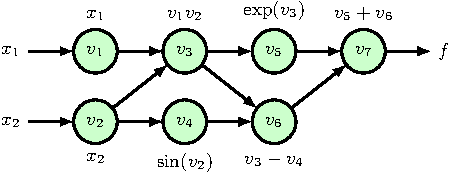
\includegraphics{Figure_4.pdf}
    \end{figure}
\end{frame}

\begin{frame}
    \frametitle{Forward-mode automatic differentiation}
    Let's define the tangent variables by $\dot{v}_{i}=\frac{\partial{}v_{i}}{\partial{}x_{1}}$. Expressions for evaluating these can be constructed automatically using the chain rule:
    \begin{equation*}
        \dot{v}_{i}=\frac{\partial{}v_{i}}{\partial{}x_{1}}=\sum_{j\in\mathrm{pa}(i)}\frac{\partial{}v_{i}}{\partial{}v_{j}}\frac{\partial{}v_{j}}{\partial{}x_{1}}=\sum_{j\in\mathrm{pa}(i)}\dot{v}_{j}\frac{\partial{}v_{i}}{\partial{}v_{j}}
    \end{equation*}
    where $\mathrm{pa}(i)$ denotes the set of parents of the node $i$ in the evaluation trace diagram. Thus for the tangent variables, we have:
    \begin{align*}
        \dot{v}_{1}&=1&\dot{v}_{2}&=0 \\
        \dot{v}_{3}&=\frac{\partial{}v_{3}}{\partial{}v_{1}}\dot{v}_{1}+\frac{\partial{}v_{3}}{\partial{}v_{2}}\dot{v}_{2}=v_{2}\dot{v}_{1}+v_{1}\dot{v}_{2}&\dot{v}_{4}&=\frac{\partial{}v_{4}}{\partial{}v_{2}}\dot{v}_{2}=\dot{v}_{2}\cos{}v_{2} \\
        \dot{v}_{5}&=\frac{\partial{}v_{5}}{\partial{}v_{3}}\dot{v}_{3}=\dot{v}_{3}\exp(v_{3})&\dot{v}_{6}&=\frac{\partial{}v_{6}}{\partial{}v_{3}}\dot{v}_{3}+\frac{\partial{}v_{6}}{\partial{}v_{4}}\dot{v}_{4}=\dot{v}_{3}-\dot{v}_{4} \\
        \dot{v}_{7}&=\frac{\partial{}v_{7}}{\partial{}v_{5}}\dot{v}_{5}+\frac{\partial{}v_{7}}{\partial{}v_{6}}\dot{v}_{6}=\dot{v}_{5}+\dot{v}_{6}
    \end{align*}
\end{frame}

\begin{frame}
    \frametitle{Forward-mode automatic differentiation}
    Now consider an example with two outputs:
    \begin{align*}
        f_{1}(x_{1},x_{2})&=x_{1}x_{2}+\exp(x_{1}x_{2})-\sin{}x_{2} \\
        f_{2}(x_{1},x_{2})&=(x_{1}x_{2}-\sin{}x_{2})\exp(x_{1}x_{2})
    \end{align*}
    We see that both $\frac{\partial{}f_{1}}{\partial{}x_{1}}$ and $\frac{\partial{}f_{2}}{\partial{}x_{1}}$ can be evaluated together in a single forward pass. But if we want to evaluate derivatives with respect to $x_{2}$ then we have to run a separate forward pass.
    \bigbreak
    In general, if we have a function with $D$ inputs and $K$ outputs then a single pass of forward-mode automatic differentiation produces a single column in the Jacobian matrix. To evaluate the full Jacobian matrix, we need $D$ forward passes. This is very efficient for networks such that $K\gg{}D$.
\end{frame}

\begin{frame}
    \frametitle{Forward-mode automatic differentiation}
    \begin{figure}
        \caption{Evaluation trace diagram for two outputs}
        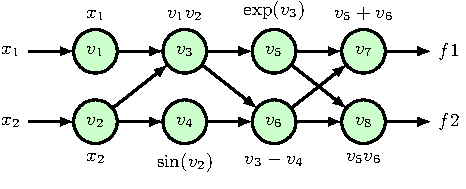
\includegraphics{Figure_5.pdf}
    \end{figure}
\end{frame}

\begin{frame}
    \frametitle{Reverse-mode automatic differentiation}
    As with forward mode, we augment each intermediate variable $v_{i}$ with additional variables, in this case called adjoint variables, denoted $\bar{v}_{i}$. For a single output function $f$, we define $\bar{v}_{i}$ as:
    \begin{equation*}
        \bar{v}_{i}=\frac{\partial{}f}{\partial{}v_{i}}
    \end{equation*}
    Using the chain rule we see that:
    \begin{equation*}
        \bar{v}_{i}=\frac{\partial{}f}{\partial{}v_{i}}=\sum_{j\in\mathrm{ch}(i)}\frac{\partial{}f}{\partial{}v_{j}}\frac{\partial{}v_{j}}{\partial{}v_{i}}=\sum_{j\in\mathrm{ch}(i)}\bar{v}_{j}\frac{\partial{}v_{j}}{\partial{}v_{i}}
    \end{equation*}
    where $\mathrm{ch}(i)$ denotes the children of node $i$ in the evaluation trace diagram.
\end{frame}

\begin{frame}
    \frametitle{Reverse-mode automatic differentiation}
    Working on the previous example again, we see that:
    \begin{align*}
        \bar{v}_{7}&=1&\bar{v}_{6}&=\frac{\partial{}v_{7}}{\partial{}v_{6}}\bar{v}_{7}=\bar{v}_{7} \\
        \bar{v}_{5}&=\frac{\partial{}v_{7}}{\partial{}v_{5}}\bar{v}_{7}=\bar{v}_{7}&\bar{v}_{4}&=\frac{\partial{}v_{6}}{\partial{}v_{4}}\bar{v}_{6}=-\bar{v}_{6} \\
        \bar{v}_{3}&=\frac{\partial{}v_{5}}{\partial{}v_{3}}\bar{v}_{5}+\frac{\partial{}v_{6}}{\partial{}v_{3}}\bar{v}_{6}=\bar{v}_{5}\exp(v_{3})+\bar{v}_{6} \\
        \bar{v}_{2}&=\frac{\partial{}v_{3}}{\partial{}v_{2}}\bar{v}_{3}+\frac{\partial{}v_{4}}{\partial{}v_{2}}\bar{v}_{4}=v_{1}\bar{v}_{3}+\bar{v}_{4}\cos{}v_{2}&\bar{v}_{1}&=\frac{\partial{}v_{3}}{\partial{}v_{1}}\bar{v}_{3}=v_{2}\bar{v}_{3}
    \end{align*}
    In general, if we have a function with $D$ inputs and $K$ outputs then a single pass of reverse-mode automatic differentiation produces a single row in the Jacobian matrix. To evaluate the full Jacobian matrix, we need $K$ reverse passes.
\end{frame}

\end{document}